% --------------------------------------------------
% DOCUMENT CLASS
% --------------------------------------------------

\documentclass[
thesis.tex
]{subfiles}

\begin{document}
	
	\newpage
	
\subsection{Impulse Response Functions}

% These are the impulse response functions of model in section \ref{sec:nk-model}. In due time, the IRF of section \ref{sec:regional-model} will be presented and a thorough analysis of the results will be conducted.

\subsubsection{Productivity Shock}

\begin{figure}[h!]
	\centering
	\begin{subfigure}[b]{0.3\textwidth}
		\centering
		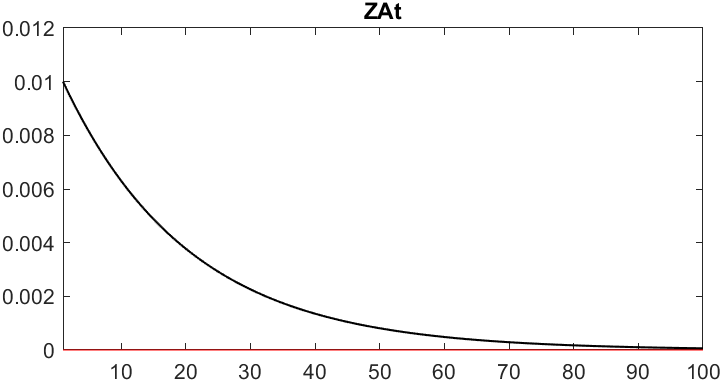
\includegraphics[width=\textwidth]{shock_ZAt/shock_ZAt_ZAt}
		\caption{Productivity Shock}
		\label{fig:zat-productivity-shock}
	\end{subfigure}
	\hfill
	\begin{subfigure}[b]{0.3\textwidth}
		\centering
		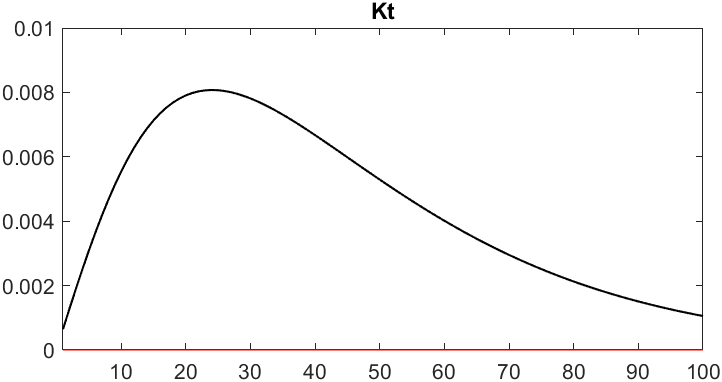
\includegraphics[width=\textwidth]{shock_ZAt/shock_ZAt_Kt}
		\caption{Capital}
		\label{fig:zat-capital}
	\end{subfigure}
	\hfill
	\begin{subfigure}[b]{0.3\textwidth}
		\centering
		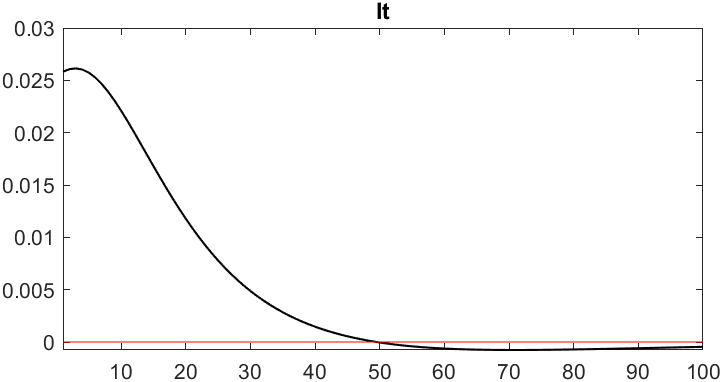
\includegraphics[width=\textwidth]{shock_ZAt/shock_ZAt_It}
		\caption{Investment}
		\label{fig:zat-investment}
	\end{subfigure}
	\hfill
	
	\vspace*{0.5cm}
	
	\begin{subfigure}[b]{0.3\textwidth}
		\centering
		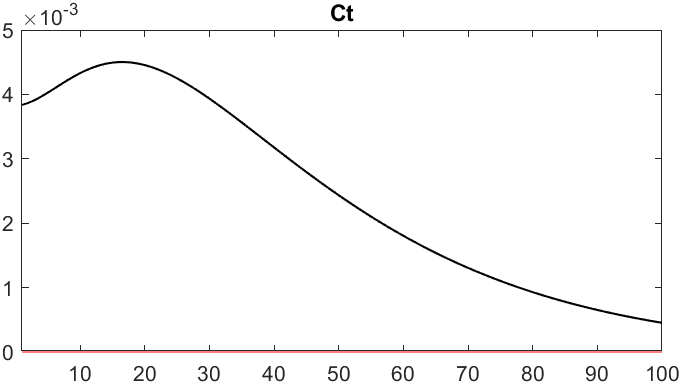
\includegraphics[width=\textwidth]{shock_ZAt/shock_ZAt_Ct}
		\caption{Consumption}
		\label{fig:zat-consumption}
	\end{subfigure}
	\hfill
	\begin{subfigure}[b]{0.3\textwidth}
		\centering
		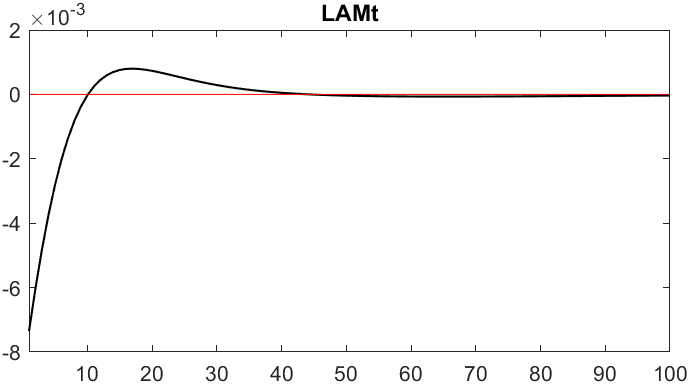
\includegraphics[width=\textwidth]{shock_ZAt/shock_ZAt_LAMBDAt}
		\caption{Marginal Cost}
		\label{fig:zat-marginal-cost}
	\end{subfigure}
	\hfill
	\begin{subfigure}[b]{0.3\textwidth}
		\centering
		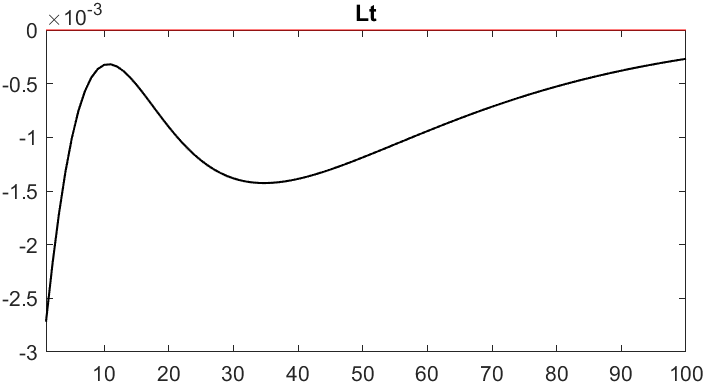
\includegraphics[width=\textwidth]{shock_ZAt/shock_ZAt_Lt}
		\caption{Labor}
		\label{fig:zat-labor}
	\end{subfigure}
	\hfill
	
	\vspace*{0.5cm}
	
	\begin{subfigure}[b]{0.3\textwidth}
		\centering
		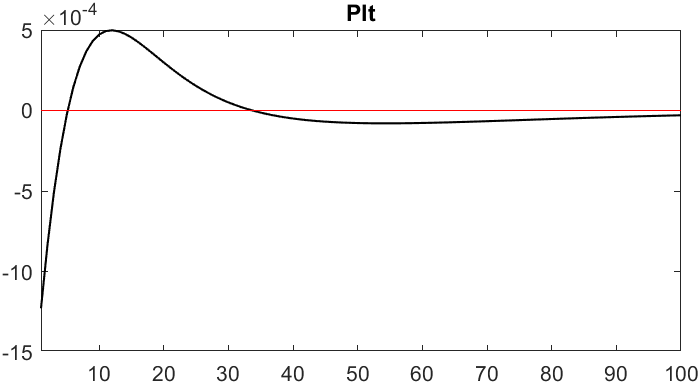
\includegraphics[width=\textwidth]{shock_ZAt/shock_ZAt_PIt}
		\caption{Inflation}
		\label{fig:zat-inflation}
	\end{subfigure}
	\hfill
	\begin{subfigure}[b]{0.3\textwidth}
		\centering
		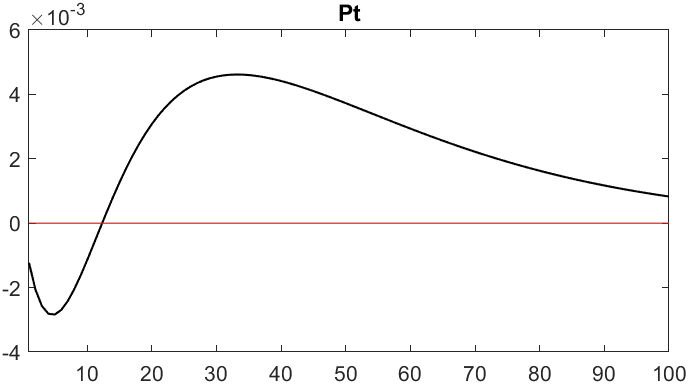
\includegraphics[width=\textwidth]{shock_ZAt/shock_ZAt_Pt}
		\caption{Price Level}
		\label{fig:zat-price}
	\end{subfigure}
	\hfill
	\begin{subfigure}[b]{0.3\textwidth}
		\centering
		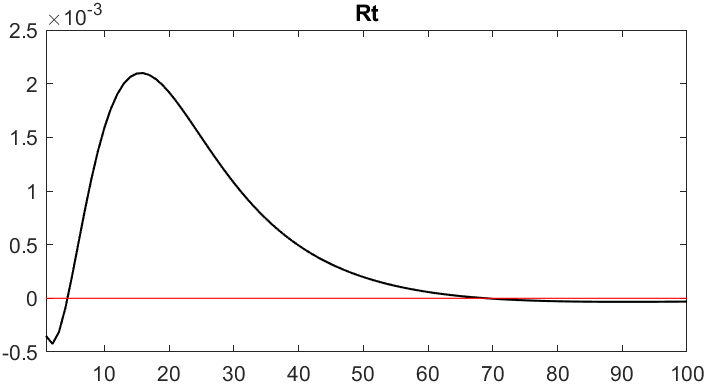
\includegraphics[width=\textwidth]{shock_ZAt/shock_ZAt_Rt}
		\caption{Interest Rate}
		\label{fig:zat-interest-rate}
	\end{subfigure}
	\hfill
	
	\vspace*{0.5cm}
	
	\begin{subfigure}[b]{0.3\textwidth}
		\centering
		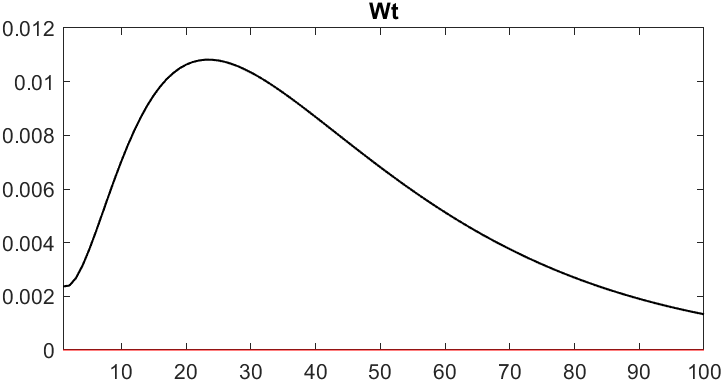
\includegraphics[width=\textwidth]{shock_ZAt/shock_ZAt_Wt}
		\caption{Wage}
		\label{fig:zat-wage}
	\end{subfigure}
	\hfill
	\begin{subfigure}[b]{0.3\textwidth}
		\centering
		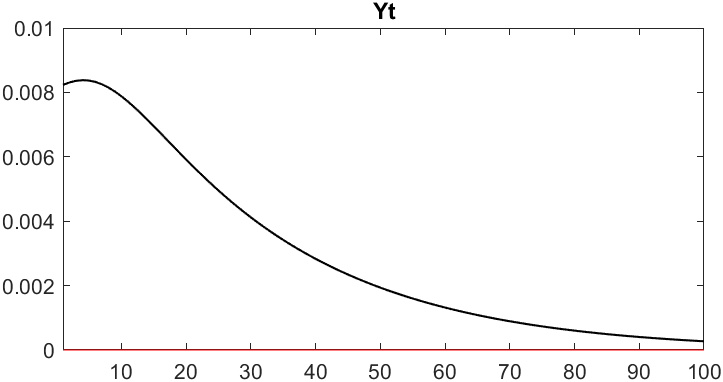
\includegraphics[width=\textwidth]{shock_ZAt/shock_ZAt_Yt}
		\caption{Production}
		\label{fig:zat-production}
	\end{subfigure}
	\hfill
	\begin{subfigure}[b]{0.3\textwidth}
		\centering
		
\includegraphics[width=\textwidth]{shock_ZAt/blank}
	\end{subfigure}
	\hfill
	\caption{Productivity Shock Impulse Response Functions}
	\label{fig:zat-irf}
\end{figure}

\newpage

\subsubsection{Monetary Shock}

\begin{figure}[h!]
	\centering
	\begin{subfigure}[b]{0.3\textwidth}
		\centering
		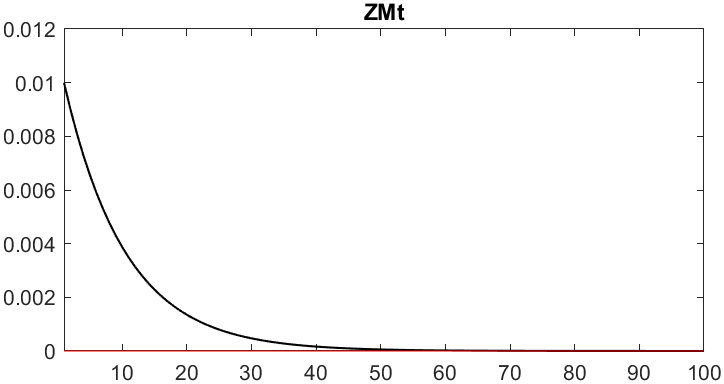
\includegraphics[width=\textwidth]{shock_ZMt/shock_ZMt_ZMt}
		\caption{Monetary Shock}
		\label{fig:ZMt-monetary-shock}
	\end{subfigure}
	\hfill
	\begin{subfigure}[b]{0.3\textwidth}
		\centering
		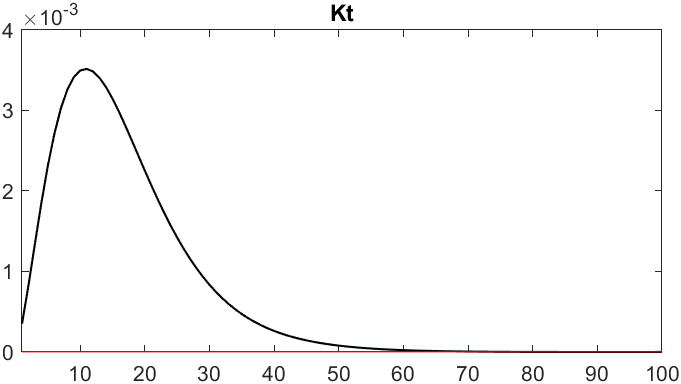
\includegraphics[width=\textwidth]{shock_ZMt/shock_ZMt_Kt}
		\caption{Capital}
		\label{fig:ZMt-capital}
	\end{subfigure}
	\hfill
	\begin{subfigure}[b]{0.3\textwidth}
		\centering
		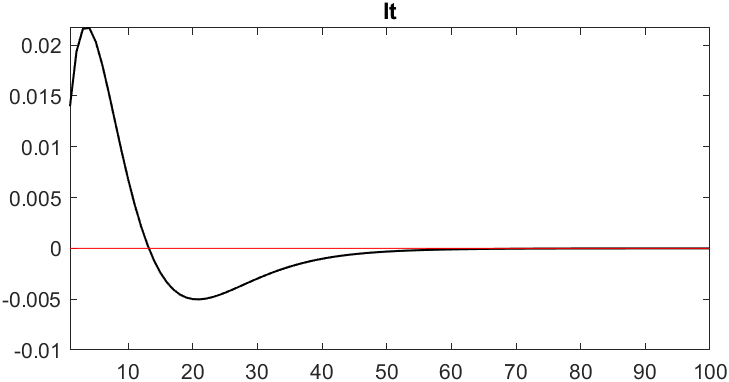
\includegraphics[width=\textwidth]{shock_ZMt/shock_ZMt_It}
		\caption{Investment}
		\label{fig:ZMt-investment}
	\end{subfigure}
	\hfill
	
	\vspace*{0.5cm}
	
	\begin{subfigure}[b]{0.3\textwidth}
		\centering
		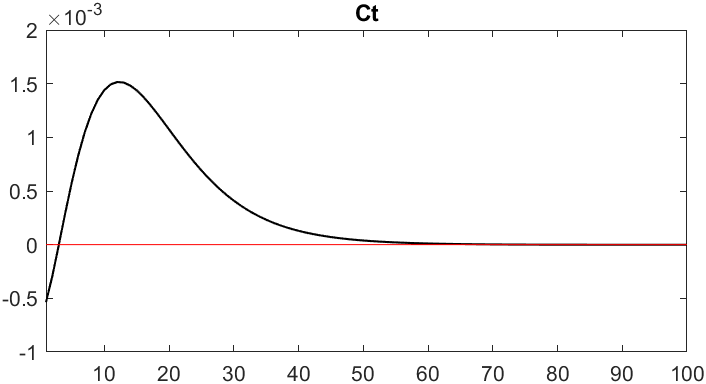
\includegraphics[width=\textwidth]{shock_ZMt/shock_ZMt_Ct}
		\caption{Consumption}
		\label{fig:ZMt-consumption}
	\end{subfigure}
	\hfill
	\begin{subfigure}[b]{0.3\textwidth}
		\centering
		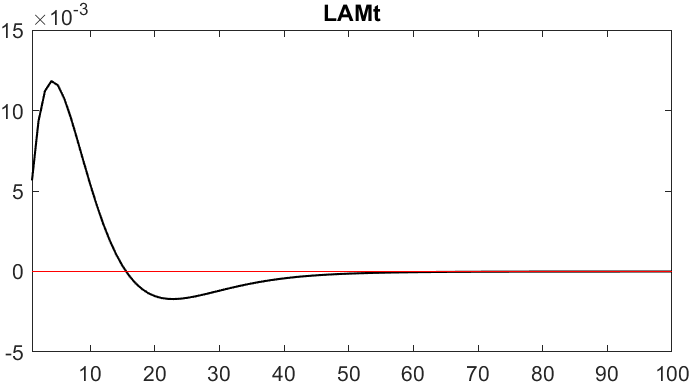
\includegraphics[width=\textwidth]{shock_ZMt/shock_ZMt_LAMBDAt}
		\caption{Marginal Cost}
		\label{fig:ZMt-marginal-cost}
	\end{subfigure}
	\hfill
	\begin{subfigure}[b]{0.3\textwidth}
		\centering
		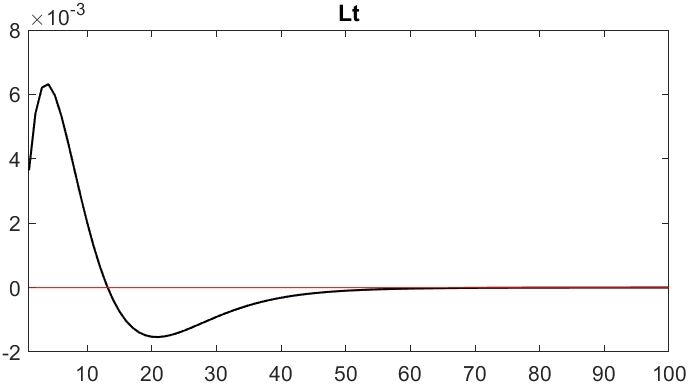
\includegraphics[width=\textwidth]{shock_ZMt/shock_ZMt_Lt}
		\caption{Labor}
		\label{fig:ZMt-labor}
	\end{subfigure}
	\hfill
	
	\vspace*{0.5cm}
	
	\begin{subfigure}[b]{0.3\textwidth}
		\centering
		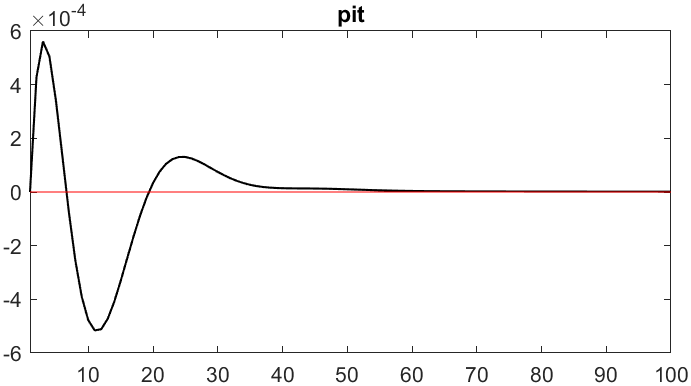
\includegraphics[width=\textwidth]{shock_ZMt/shock_ZMt_PIt}
		\caption{Inflation}
		\label{fig:ZMt-inflation}
	\end{subfigure}
	\hfill
	\begin{subfigure}[b]{0.3\textwidth}
		\centering
		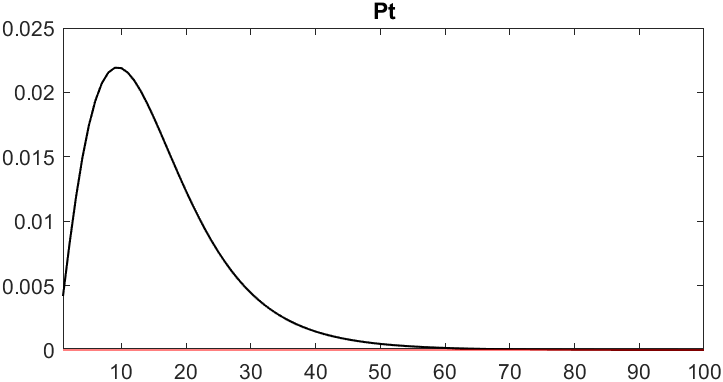
\includegraphics[width=\textwidth]{shock_ZMt/shock_ZMt_Pt}
		\caption{Price Level}
		\label{fig:ZMt-price}
	\end{subfigure}
	\hfill
	\begin{subfigure}[b]{0.3\textwidth}
		\centering
		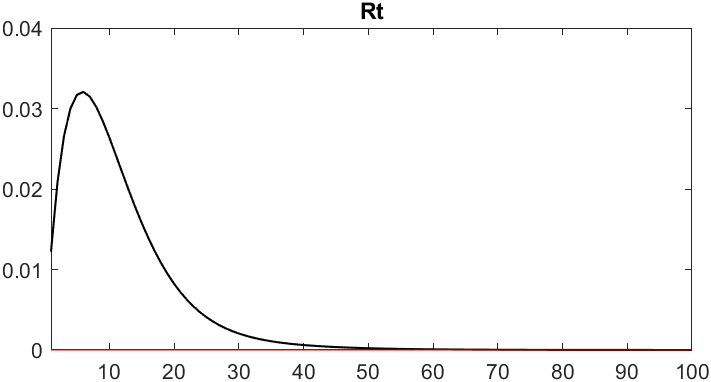
\includegraphics[width=\textwidth]{shock_ZMt/shock_ZMt_Rt}
		\caption{Interest Rate}
		\label{fig:ZMt-interest-rate}
	\end{subfigure}
	\hfill
	
	\vspace*{0.5cm}
	
	\begin{subfigure}[b]{0.3\textwidth}
		\centering
		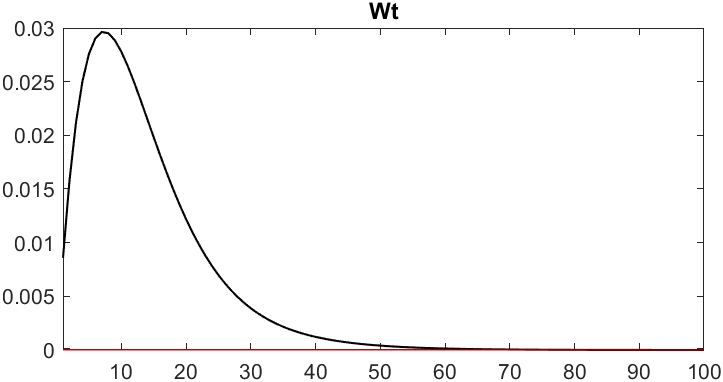
\includegraphics[width=\textwidth]{shock_ZMt/shock_ZMt_Wt}
		\caption{Wage}
		\label{fig:ZMt-wage}
	\end{subfigure}
	\hfill
	\begin{subfigure}[b]{0.3\textwidth}
		\centering
		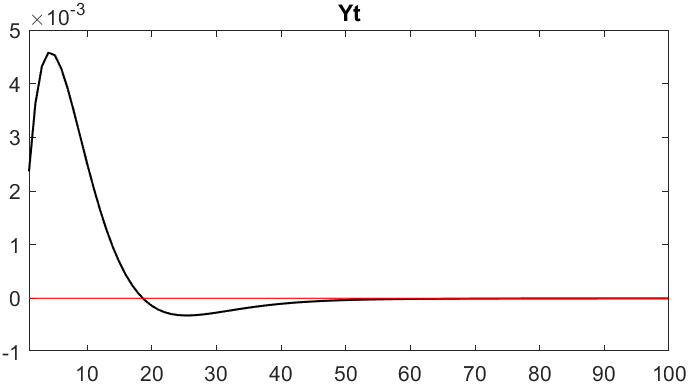
\includegraphics[width=\textwidth]{shock_ZMt/shock_ZMt_Yt}
		\caption{Production}
		\label{fig:ZMt-production}
	\end{subfigure}
	\hfill
	\begin{subfigure}[b]{0.3\textwidth}
		\centering
		
\includegraphics[width=\textwidth]{shock_ZMt/blank}
	\end{subfigure}
	\hfill
	\caption{Monetary Shock Impulse Response Functions}
	\label{fig:ZMt-irf}
\end{figure}

\end{document}